\section[Pseudo-spectral]{The pseudo-spectral method} \label{sec:pseudospectral}

\subsection{Introduction} \label{sec:lag_intro}
The Navier-Stokes equations are 
\begin{equation} \label{eq:navier-stokes}
  \partial_t \vec{u} + u\cdot\vec{\nabla} \vec{u} = -\vec{\nabla} p +\nu \Delta \vec{u} + \vec{f}
\end{equation}
where $\Delta$ is the Laplacian operator and the density $\rho$ is absorbed redefining $p$ as $p/\rho$ and $\nu$, the kinematic viscosity, as $\mu/\rho$ (here $\mu$ is the dynamic viscosity). $f_i$ is a forcing term, necessary to keep the fluid moving, balancing the dissipative term.

No exact solutions have been found for these equations yet, as well as their existence and uniqueness has not been proved, making it a noteworthy problem in theoretical physics, despite being classical physics. Nevertheless, some qualitative and quantitative results help characterizing the phenomenon known as \textit{turbulence}. Defining turbulence is somehow difficult, since it refers to the chaotic motion of fluids when the inertial forces dominate viscous ones, as the Reynold's number 
\[ Re \coloneqq \frac{UL}{\nu} \]
parametrizes ($U$ and $L$ are some characteristic velocity and length, respectively) \autocite{frisch}. The meaning of this number is to be found with its dimensional analysis: \( Re \propto \frac{u\cdot\vec{\nabla} \vec{u}}{\nu \Delta \vec{u}} \) so it represents the ratio between inertial and viscous forces. Its value in the simulations is \(Re \sim 310\). When making the variables non-dimensional,
\[ u \rightarrow \frac{u}{U} \;\;;\;\;\; l \rightarrow \frac{l}{L} \;\;;\;\;\; t \rightarrow \frac{t}{L/U} \]
\autoref{eq:navier-stokes} can be rewritten as
\[   \partial_t \vec{u} + u\cdot\vec{\nabla} \vec{u} = -\vec{\nabla} p + \frac{1}{Re} \Delta \vec{u} + \vec{f'} \]
showing, according to the \textit{principle of similarity}, that Reynold's number is the only control parameter (given the boundary conditions). In \autoref{fig:vandyke} an example of turbulent motion is shown. 

In \autoref{tab:3dparam} some typical parameters of the simulation are shown: the characteristic dimension of the dissipative scale \(\eta = \left(\frac{\nu^3}{\epsilon}\right)^{1/4}\), its characteristic time \( \tau_\eta = \left(\frac{\nu}{\epsilon}\right)^{1/2}\), and the large-scale time \( T = \frac{u_{RMS}^2}{\epsilon} \); the spatial resolution of the spacial discretization.

\begin{table}
\centering
\begin{tabular}{c|c}
$Re$ & 310 \\ \hline
$\eta$ & 0.07 \\ \hline
$\tau_\eta$ & 0.36 \\ \hline
$T$ & 3.6 \\ \hline
spatial resolution & $128^3$ \\ \hline
grid spacing & 0.05 
\end{tabular}
\caption{}
\label{tab:3dparam}
\end{table}

\begin{figure}
    \centering
    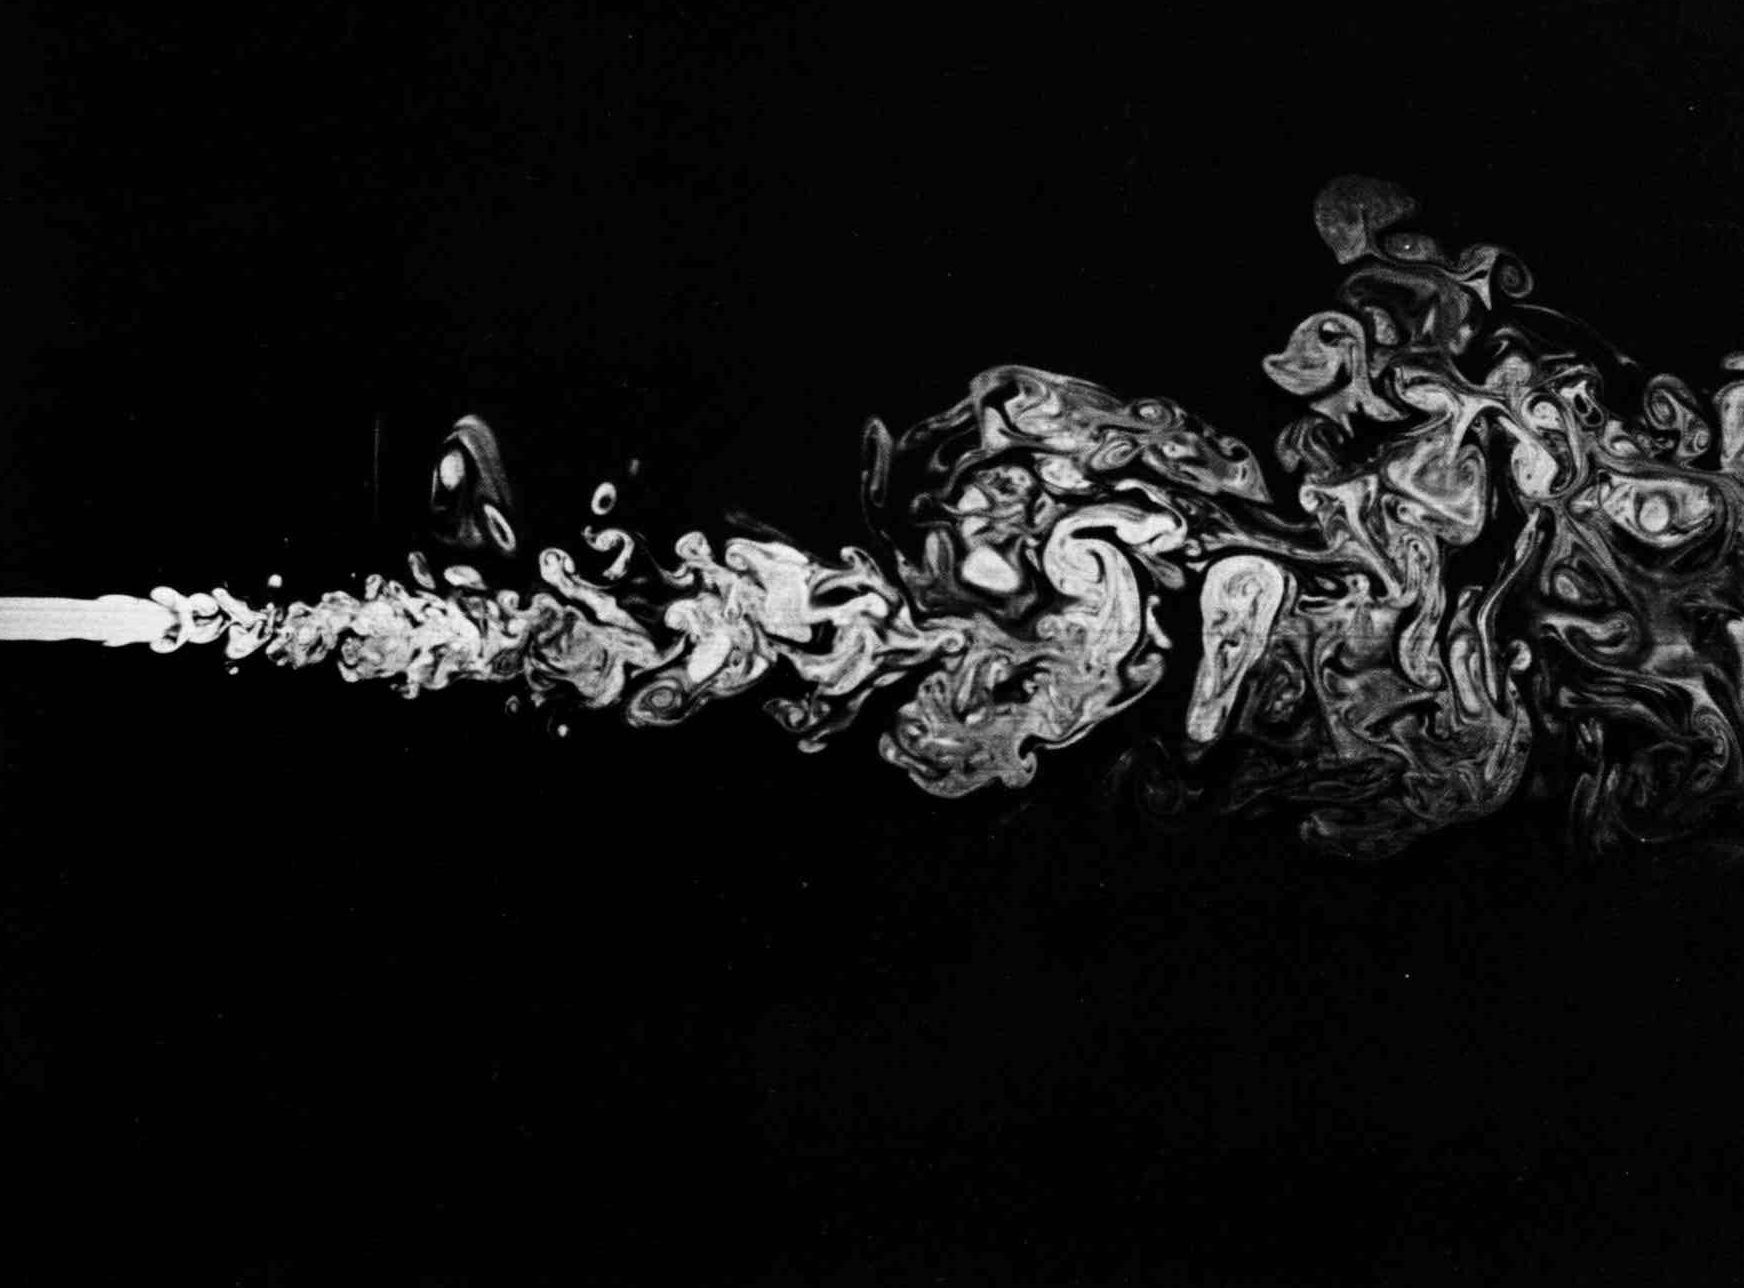
\includegraphics[width=\textwidth]{img/turb_flow_VanDyke}
    \caption{A Re=2300 turbulent water jet. [Image adapted from \autocite{van1982album}.]}
    \label{fig:vandyke}
\end{figure}

In \autocite[chapter 5.2]{frisch}, the following reasoning is developed: when a fluid exerts a force on an object (which will be assumed cilindrical, for sake of simplicity), it will hold the dimensional proportionality
\[ F \propto \rho S U^2 \]
(where $\rho$ is a density, $S$ is an area, $U$ is a velocity), so that the work is
\[ W = FU \propto \rho S U^3 \]
and the kinetic energy dissipated per unit mass is
\[ \epsilon = \frac{W}{\rho L^3 } \propto \frac{U^3}{L} \]
A more rigorous treatise looks at the structure function:
\[ \langle \left( \delta u_\parallel \right)^2 \rangle \propto \epsilon^{2/3} l^{2/3} \]
where \( \delta u_\parallel \coloneqq \left[\vec{u}(\vec{r}+\vec{l}) - \vec{u}(\vec{r})\right]\cdot \frac{\vec{l}}{l} \). 

A method to solve these equations is said to be \textit{spectral} when working in Fourier space, so that the non-locality that would be induced by the derivatives is avoided. The present method is called \textit{pseudo-spectral} to point out the approach used to computed the product of two Fourier-transformed elements, which would normally require a convolution: a sequence of FT (Fourier-transform) and anti-FT is used instead to compute the product in the physical space.

In order to see turbulence the recommended range is \( k_{max}\eta= 1.5\div2 \), since this means that \( \frac{\eta}{\lambda_{min}} \gtrsim \frac{1.5}{2\pi} \) and the Kolmogorov length is reached. Since \( k_{max} = \frac{2}{3} \frac{N_{grid points}}{2} \frac{2\pi}{L} \) where $L$ is the size of the grid, it is fixed by the chosen resolution $\frac{N_{grid points}}{L}$. Given a dissipation $\epsilon$, the only free variable left is $\nu$, which determines the Kolmogorov length \(\eta=\left(\frac{\nu^3}{\epsilon}\right)^{1/4}\).

\subsection{The equations}
Considering \autoref{eq:navier-stokes}, some conditions are necessary to come to a solution. 
\subsubsection{Incompressibility}
First of all, the fluid is assumed to be \textit{incompressible}, a condition reflected in the flow being solenoidal (\(\mathrm{div} \vec{u} = 0\)), as can be seen from continuity equation: \(\partial_t \rho + \vec{\nabla} \cdot(u\rho) =0 \).
The velocity flow can be thus expressed with a vector potential: \( \vec{u} = \mathrm{rot} \vec{b} \). The gauge \(\mathrm{div} \vec{b} = 0 \) is imposed. 
\autoref{eq:navier-stokes} becomes
\begin{equation} \label{eq:ns-vecpot-pre}
  \partial_t \vec{b} + \mathrm{rot}^{-1} (\vec{u}\cdot\vec{\nabla}\vec{u}) = \mathrm{rot}^{-1} (\vec{\nabla}p) +\nu\;\mathrm{rot}^{-1}\Delta\vec{u} + \mathrm{rot}^{-1} \vec{f}
\end{equation}
Some simplifications are possible:
\begin{itemize}
  \item The vorticity can be defined as \( \vec{\omega} := \mathrm{rot} \vec{u}\). In the chosen gauge, \( \omega_i = -\partial^2 b_i \) and inverting the definition of $b$ it follows the following symbolic equivalence between operators 
    \[ \mathrm{rot}^{-1} \doteq \Delta^{-1} \mathrm{rot} \]
    A consequence is that the term containing pressure vanishes, since the rotor of a gradient is always zero.
  \item Since the locality is guaranteed by the use of FT, the Laplacian operator and the rotor commute
\end{itemize}
The equations become
\begin{equation} \label{eq:ns-vecpot}
  \partial_t \vec{b} + \mathrm{rot}^{-1} (\vec{u}\cdot\vec{\nabla}\vec{u}) = \nu\;\Delta\vec{b} + \vec{f_b}
\end{equation}
For the sake of brevity, the following definitions are given:
\[ \mathrm{NLT}(\vec{x}) = \mathrm{rot}^{-1}
(\vec{u}\cdot\vec{\nabla}\vec{u}) \;\;;\;\;\; 
\mathrm{VISC}(\vec{x}) = \nu\;\Delta\vec{b} \]
which stand for "Non-Linear Term" and "Viscous Term".

\subsubsection{Evaluation of NLT}
The non-linear term (NLT) contains a product, which in Fourier space would convert in a convolution, implying a high computational cost ($~N^2$); instead an anti-FFT can be performed to bring the product back to physical space, where just $N$ steps are required, so that the whole operation involves \( N + N\log N\) steps.

%\subsubsection{Boundary conditions}
%Periodic boundary conditions allow a simple inversion of Laplacian operator. ...

\subsection{Discretization}
Considering \autoref{eq:ns-vecpot}, it turns out to be favourable to transform it to the momentum space\footnote{The symbols \( \widehat{\bullet} (\vec{k}) \coloneqq \mathcal{F}[\bullet(\vec{x})] \) refer to the Fourier transform}:
\begin{equation} \label{eq:ns-vecpot-four}
\partial_t \widehat{\vec{b}} = \widehat{\mathrm{NLT}}(\vec{k}) - \nu k^2 \widehat{\vec{b}} + \vec{\widehat{f}}(\vec{k})
\end{equation}
In order to simplify it the forcing is considered separately from the rest of the equation, which is solved as follows.
Defining \( \vec{g} \coloneqq \widehat{\vec{b}} e^{\zeta t} \), where \( \zeta \coloneq \nu k^2 \), applying the product rule for derivatives and using \autoref{eq:ns-vecpot-four}
\[ \partial_t \vec{g} = \widehat{\mathrm{NLT}} e ^{\zeta t} \]
A second-order Runge-Kutta scheme is used to solve for $g$, referring to \autoref{eq:RK2_halfstep} and resulting in  
\begin{equation}
  \begin{cases} 
    t_{n+1/2} = t_n + \dt/2 & \\
    g_{n+1/2} =  g_n + \frac{\dt}{2}\widehat{\mathrm{NLT}}_n &\\
    g_{n+1} = g_n + \frac{\dt}{2}\widehat{\mathrm{NLT}}_{n+1/2} &\\
  \end{cases}
\end{equation}
which returning to $\vec{b}$ leads to
\begin{align}
\vec{b}_{n+1} &= \vec{g}_{n+1} e^{-\zeta(t+\dt)} \\
              &= \vec{b}_n e^{-\zeta \dt} +
\widehat{\mathrm{NLT}}_{n+1/2} e^{-\zeta\frac{\dt}{2} } \frac{\dt}{2} \end{align}


%\subsubsection{FFT and aliasing}
%The reference used to discuss this is \cite[chapter 12]{num_rec}: 

%\subsubsection{Forcing}
